\documentclass{foi}
\usepackage{lipsum}
\usepackage{subcaption}

\vrstaRada{\zavrsni} % \diplomski
\title{Kontrola pristupa koristeći informacije iz kreditnih kartica}

\author{Mate Nakić}
\spolStudenta{\musko} % \zensko ili \musko
\mentor{Boris Tomaš}
\spolMentora{\musko} % \zensko ili \musko
\godina{2021}
\mjesec{kolovoz}
\date{2021}
%\status{redoviti}
\indeks{44880/16-R}
\smjer{Informacijski sustavi} % (ili Poslovni sustavi, Ekonomika poduzetništva, Primjena informacijske tehnologije u poslovanju, Informacijsko i programsko inženjerstvo, Baze podataka i baze znanja, Organizacija poslovnih sustava, Informatika u obrazovanju)
\titulaProfesora{doc. dr. sc.}

\sazetak{Opsega od 100 do 300 riječi. Sažetak upućuje na temu rada, ukratko se iznosi čime se rad bavi, teorijsko-metodološka polazišta, glavne teze i smjer rada te zaključci.}

\kljucneRijeci{riječ; riječ; ...riječ; Obuhvaća 7+/-2 ključna pojma koji su glavni predmet rasprave u radu.}

\begin{document}

\maketitle

\tableofcontents

\pagestyle{plain}

\chapter{Uvod}

Svakim danom svijet se sve više digitalizira i mehanički procesi se automatiziraju kako bi se uštedjelo na vremenu i resursima.
Sve više smo svjesni koliko računala lako i s manje grešaka obavljaju ponavljajuće zadatke, za razliku od ljudi.
Jedan od ponavljajućih i sklon pogrešci zadatak jest kontrola i evidencija pristupa.
Proces zahtjeva dva sudionika: kontrolora i korisnika.
U tradicionalnom (ne-digitaliziranom) okruženju kontrolor je osoba koja prima zahtjeve korisnika, prema određenim uvjetima
dozvoljava ili odbija pristup korisniku te evidentira u evidencijsku knjigu komu i kad je pristup dozvoljen ili odbijen.
Proces je vrlo jednostavan, no ima više prostora za pogrešku:
\begin{itemize}
    \item Je li kontrolor prisutan?
    \item Jesu li uvjeti stvarno ispunjeni (zloupotreba ovlasti ili ljudska greška)?
    \item Jesu li podaci korisnika ispravni (npr.\ ime i prezime)?
    \item Jesu li meta podaci ispravni (npr.\ datum i vrijeme)?
\end{itemize}
Digitalizacijom ovog procesa kontrolor više nije osoba već uređaj, evidencijska knjiga nije list papira nego oblak (eng. \textit{cloud}).
Ista pitanja mogu biti postavljena nakon digitalizacije, no vjerojatnost pogreške je znatno manja.

Praktični dio rada je implementacija kontrole pristupa (eng. \textit{access control}) pomoću potrošačkih elektroničkih
komponenti (eng. \textit{consumer electronics}), oblaka i kreditnih kartica.
Elektroničke komponente tvore uređaj (kontrolor) u obliku sefa s kojim korisnik komunicira dok kreditna kartica služi kao sredstvo identifikacije.
U oblaku se nalazi aplikacija u kojoj se definiraju kreditne kartice koje imaju pravo pristupa.
Uspješni i neuspješni pokušaji pristupanju se evidentiraju u bazu podataka u oblaku.

\section{Hipoteze i ciljevi}

Sljedeće su hipoteze:

\begin{itemize}
    \item \textbf{H1}: Može se pročitati jedinstveni identifikator kreditne kartice bez narušavanja privatnosti (čitanje osobnih podataka).
    \item \textbf{H2}: Moguće je stvoriti kontrolni uređaj pomoću potrošačke elektronike.
    \item \textbf{H3}: Internet protokolima je moguće delegirati logiku autoriziranja na udaljeni server.
\end{itemize}

Ciljevi rada su:

\begin{itemize}
    \item \textbf{C1}: Razviti pločicu s mikrokontrolerom i potrebnim perifernim komponentama.
    \item \textbf{C2}: Smjestiti pločicu i komponente u sef.
    \item \textbf{C3}: Omogućiti konfiguriranje bežične pristupne točke sefa.
    \item \textbf{C4}: Definirati infrastrukturu u oblaku.
    \item \textbf{C5}: Razviti grafičko sučelje na web platformi za upravljanje dozvolama i pregledavanje povijesti otvaranja.
    \item \textbf{C6}: Razviti pozadinsku aplikaciju na web platformi za obrađivanje autorizacijskih zahtjeva sefa.
    \item \textbf{C7}: Ostvariti komunikaciju sefa i udaljenog servera pomoću HTTP protokola.
    \item \textbf{C8}: Zabilježiti svaki pokušaj autoriziranja (uspješan ili neuspješan) na udaljenom serveru.
\end{itemize}


\chapter{Pregled literature}

\ldots


\chapter{Web aplikacija}

Sustav kontrole i evidencije pristupa viđen s visoke razine sastoji se od tri cjeline:
\begin{itemize}
    \item Infrastruktura
    \item Pozadinska aplikacija
    \item Grafičko sučelje
\end{itemize}

U ovom poglavlju sve tri cjeline će biti opisane i razrađene.

\section{Infrastruktura}
Infrastruktura je sačinjena od servera, čvorova, usmjerivača i sl.
Također, infrastrukturu čini operacijski sustav, vatrozid, i ostali softver\cite{ibm-infrastructure}.
Po tom pitanju danas se ništa značajno nije promijenilo, samo su fizičke komponente skrivene u "oblaku" (eng. \textit{cloud}).
Rad zahtjeva vrlo jednostavnu infrastrukturu pa je oblak prikladno rješenje jer ne zahtjeva vlastoručnu konfiguraciju i održavanje fizičkih komponenti.

\begin{figure}[h!]
    \centering
    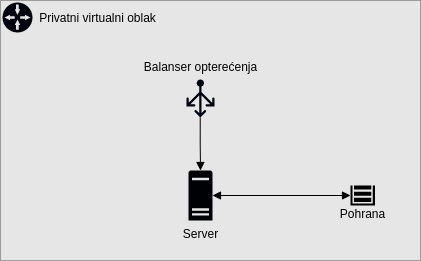
\includegraphics[scale=0.7]{images/infrastructure}
    \caption{Fizičke komponente infrastrukture}
    \label{fig:physical-infrastructure}
\end{figure}

Na slici~\ref{fig:physical-infrastructure} nalaze se sve komponente kreirane kod pružatelja usluge oblaka (DigitalOcean).
Privatni virtualni oblak ima mnoštvo značajki, ali u ovom slučaju se koristi samo za logičko grupiranje komponenti.
Balanser opterećenja (eng. \textit{load balancer}) služi kao \textit{proxy} do glavnog servera i moguće je povezati domenu na njega.
Server ima vlastitu sekundarnu pohranu na kojoj se nalazi operacijski sustav i potrebni alati ali i vanjsku pohranu na kojoj se nalaze aplikacijski podaci.

Vanjska pohrana i balanser opterećenja izgledaju, na prvi pogled, nepotrebni.
U scenariju kad se glavni server nepovratno sruši vrlo je lako kreirati novi i nastaviti s normalnim radom.
Krajnji korisnik osjeti kratki prekid usluge, a ne potpuni gubitak usluge i podataka.
U slučaju samo jednog servera (bez vanjske pohrane i balansera opterećenja) podaci i IP adresa se trajno gube što predstavlja veliku
neugodnost krajnjem korisniku.

\subsection{Infrastruktura aplikacije}

Moderne aplikacije zahtijevaju različite servise i alate kako bi funkcionirale u potpunosti.
Baza podataka, red čekanja, posrednik poruka i web server samo su neki od servisa.
Potrebni su alati za ažuriranje, objavljivanje i nadzor aplikacija i servisa.

Danas je najpopularniji način objavljivanja aplikacija pomoću kontejnera.
Kontejner je rezultat procesa pakiranja aplikacijskog koda sa svim potrebnim bibliotekama i alatima kako bi ga se moglo
lako i pouzdano prenositi između okruženja, npr.\ lokalno (na računalu programera), testno (\textit{staging}) i
stvarno (\textit{production})~\cite{docker-containers}.

Sam kontejner nema nikakvu funkciju dok se ne pokrene.
Kontejneri nisu izvršne datoteke (\textit{.exe}) da ih operacijski sustav može pokrenuti bez dodatnih alata.
Čak i kad bi operacijski sustav to mogao, kontejner je moguće zaustaviti, ponovno pokrenuti, može završiti u stanju
greške (eng. \textit{error state}) te je potrebna "logika" kad i kako treba poduzeti određene akcije.
Operacijski sustav se bavi puno nižim stvarima pa problem upravljanja kontejnerom izlazi iz domene operacijskog sustava.

Aplikacije su uglavnom sačinjene od više modula i servisa pa je potrebno i više kontejnera.
Ručno upravljanje s istima je vremenski i resursno zahtjevan proces, ali postoje alati koji olakšavaju upravljanje kontejnerima.
To su alati koji pomažu pri orkestriranju kontejnera (eng. \textit{container orchestration}) i jedan od njih je i \textit{Kubernetes}.
Kubernetes je sustav koji pomaže pri automatiziranju procesa objave i ažuriranja, skaliranja i sveukupnog
upravljanja aplikacijama i servisima~\cite{kubernetes}.

Razmjer praktičnog rada ne zahtjeva mnoštvo značajki koje Kubernetes nudi, samo osnovnu značajku:
grupira kontejnere koji čine aplikaciju u logičke jedinice~\cite{kubernetes}.
To omogućava lakše razumijevanje komponenti sustava kao i vizualizaciju istih.

\pagebreak

\begin{figure}[h!]
    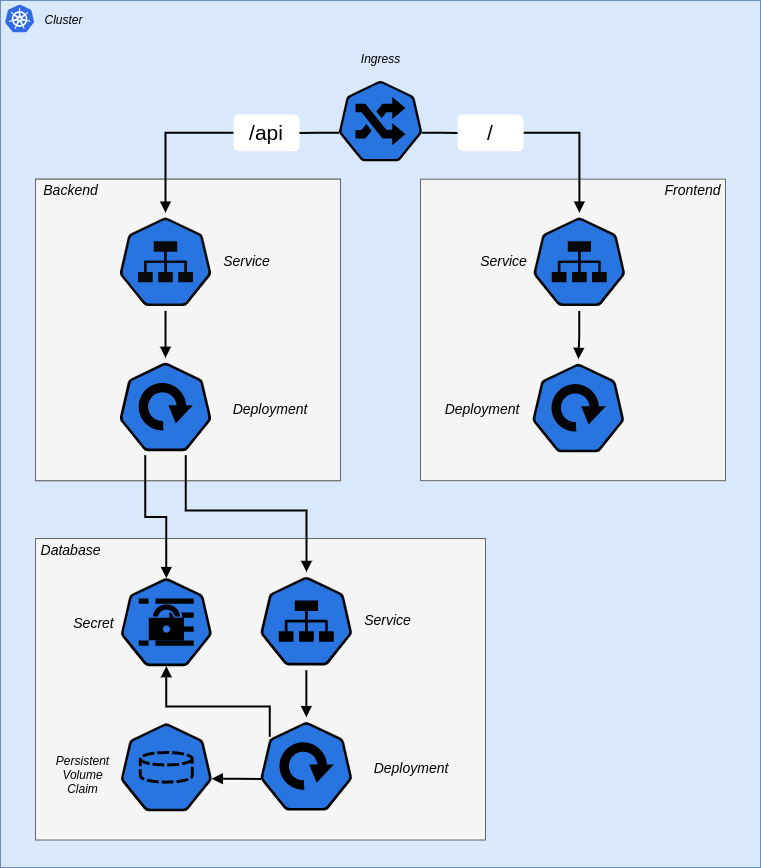
\includegraphics[width=\textwidth]{images/app-infrastructure}
    \caption{Servisi i komponente sustava}
    \label{fig:application-infrastructure}
\end{figure}

Na slici~\ref{fig:application-infrastructure} je prikazan \textit{cluster} sa svim servisima i komponentama.
Početna točka je \textit{ingress} koji funkcionira kao \textit{proxy}.
Ovisno o putanji koju korisnik zahtjeva, zahtjev se prosljeđuje na \textit{backend} (pozadinska aplikacija) ili \textit{frontend} (grafičko sučelje).

Grafičko sučelje se sastoji od dvije komponente: \textit{Service} i \textit{Deployment}.
\textit{Deployment} zna kako pokrenuti kontejner, kad je kontejner spreman za obradu zahtjeva i koliko replika ima.
Kako svaki kontejner ima svoju IP adresu ostali servisi bi morali znati točnu IP adresu kontejnera
kako bi ga mogli koristiti.
\textit{Service} predstavlja apstrakciju nad kontejnerima i ponaša se kao balanser opterećenja (u slučaju više replika)
ili \textit{proxy} (u slučaju jedne replike).

Pozadinska aplikacija je slična grafičkom sučelju osim što ovisi o bazi podataka.
Ovisi o \textit{Service} komponenti baze podataka kao i pristupnim podacima koji se nalaze u komponenti \textit{Secret}.
Kako bi pozadinska aplikacija komunicirala s bazom podataka potrebno je nekoliko podataka:
\begin{itemize}
    \item Adresa
    \item Korisničko ime
    \item Lozinka
    \item Naziv baze podataka
\end{itemize}

Kako je već rečeno da je \textit{Service} apstrakcija nad kontejnerima tako je sam naziv servisa ujedno i \textbf{adresa}.
\textbf{Korisničko ime}, \textbf{lozinka} i \textbf{naziv baze podataka} se nalaze u \textit{Secret} komponenti.
Ona predstavlja jedini izvor točnosti (eng. \textit{single source of truth}) pa ukoliko dođe do promjena
u podacima pozadinska aplikacija i baza podataka mogu pravilno reagirati kako bi nesmetano funkcionirali.

Baza podataka, naspram pozadinske aplikacije, ima jednu komponentu više: \textit{Persistent Volume Claim}.
Svaki kontejner ima sustav datoteka odvojen od domaćinovog sustava datoteka (eng. \textit{host file system}).
U slučaju zaustavljanja kontejnera (namjerno ili uslijed greške) svi podaci bi bili trajno izgubljeni.
Kako bi se to izbjeglo potrebno je dozvoliti kontejneru pisanje u domaćinov sustav datoteka.
Komponenta \textit{Persistent Volume Claim} apstrahira ovu funkcionalnost pa sam kontejner uopće ne zna da se podaci zapravo
zapisuju na domaćinov sustav datoteka.
To omogućava djelomično fizičko odvajanje domaćinovog sustava datoteka.
Direktoriji koji su potrebni bazi podataka su odvojeni na vanjsku pohranu (slika~\ref{fig:physical-infrastructure}) dok su
podaci i datoteke o kojima ovisi operacijski sustav pohranjeni na internu pohranu servera.
U slučaju nepovratnog pada servera (npr.~fizičko oštećenje) zamjenom servera sustav nastavlja raditi bez gubitka podataka.


\section{Pozadinska aplikacija}
Pozadinska aplikacija definira većinski dio logike sustava.
Svoje funkcionalnosti daje na korištenje kroz REST API kako bi grafičko sučelje i sef mogli ispunjavati svoje uloge.
Funkcionalnosti su sljedeće:

\begin{itemize}
    \item Upravljanje karticama
    \item Autorizacija kartica
    \item Pregled evidencije (ne)autoriziranih kartica
    \item Autorizacija korisnika
\end{itemize}

Funkcionalnosti su implementirane u programskom jeziku \textit{PHP} uz pomoć \textit{Laravel} radnog okvira.

\subsection{Upravljanje karticama}

Entitet "Kartica" sadrži podatke o imenu kartice i jedinstvenom identifikatoru (\textit{UID}).
Sadrži i meta podatke o datumu stvaranja i datumu izmjene.
Entitetom korisnik upravlja kroz grafičko sučelje, a pozadinska aplikacija koristi jedinstvene identifikatore pri autoriziranju
zahtjeva sefa.

Entitet kartice nema relacija na druge entitete pa nema smisla prikazivati ER dijagram već je dovoljan programski kod.
Radni okvir omogućava definiranje migracija baze podataka kroz programski jezik umjesto pisanja čistog SQL-a.

\begin{lstlisting}[language=PHP]
class CreateCardsTable extends Migration
{
    public function up()
    {
        Schema::create('cards', function (Blueprint $table) {
            $table->id();
            $table->string('name')->unique();
            $table->string('uid')->unique();
            $table->timestamps();
        });
    }

    public function down()
    {
        Schema::dropIfExists('cards');
    }
}
\end{lstlisting}

Radni okvir ima ORM (\textit{Object Relational Mapper}) zvan \textit{Eloquent} što omogućava rad s bazom kroz objekte
umjesto ručnog pisanja SQL upita.
Dovoljno je definirati klasu prema imenu tablice, u jednini, i naslijediti klasu \textit{Model} iz radnog okvira.

\begin{lstlisting}[language=PHP]
class Card extends Model
{
    static function existsByUid(string $uid)
    {
        return static::query()->where('uid', '=', $uid)->exists() === true;
    }
}
\end{lstlisting}

Statična metoda \textit{existsByUid} provjerava postoji li zapis kartice s danim \textit{UID-em} i vraća \textit{true} ili \textit{false}.
Ona je osnovica za autorizacijske zahtjeve sefa.

\pagebreak

Operacije nad entitetom kartice su izložene (dane na korištenje) vanjskom svijetu, odnosno grafičkom sučelju kroz niz
HTTP putanji:

\begin{table}[h!]
    \centering
    \caption{Prikaz putanja svih funkcionalnosti upravljanja karticama}
    \begin{tabularx}{\textwidth}{|X|X|X|}
        \hline
        \cellcolor{gray!25} Funkcionalnost & \cellcolor{gray!25} HTTP Metoda + Putanja & \cellcolor{gray!25} Klasa@Metoda \\
        \hline
        Popis svih kartica & GET /api/card & CardController@index \\
        \hline
        Stvaranje kartice & POST /api/card & CardController@store \\
        \hline
        Uređivanje kartice & PUT /api/card/\{id\} & CardController@update \\
        \hline
        Brisanje kartice & DELETE /api/card/\{id\} & CardController@destroy \\
        \hline
    \end{tabularx}
    \\[10pt]
    \label{tab:card_functionalities}
\end{table}

Iz tablice~\ref{tab:card_functionalities} može se vidjeti da sve funkcionalnosti dijele isti dio putanje URL-a: \textbf{/api/card}
kao i istu klasu u kojoj su implementirane metode: \textbf{CardController}.
Kako su \textit{Create, Read, Update, Delete (CRUD)} operacije nad istim entitetom ponavljajući uzorak u većini aplikacija, radni okvir omogućava
jednostavno definiranje putanja i pripadnih metoda:

\begin{lstlisting}[language=PHP]
Route::resource('card', CardController::class)->only(['index', 'store', 'update', 'destroy']);
\end{lstlisting}

Prema tablici~\ref{tab:card_functionalities} popis svih kartica je implementiran u metodi \textbf{index}.
Jednostavan upit dohvaća osnovne podatke o karticama, sortira ih po datumu stvaranja i vraća u JSON formatu.

\begin{lstlisting}[language=PHP]
public function index(): JsonResponse
{
    $cardsByCreationDateAscending = Card::query()->select(['id', 'name', 'uid'])->orderBy('created_at')->get();

    return response()->json([
        'data' => $cardsByCreationDateAscending
    ]);
}
\end{lstlisting}

Prema tablici~\ref{tab:card_functionalities} stvaranje nove kartice je implementiran u metodi \textbf{store}.
Metoda stvara objekt \textit{Card} i popunjava ga s podacima danih od strane korisnika.
Kod uspješnog spremanja vraćaju se svi podaci o kartici u JSON formatu, a kod neuspješnog spremanja vraća se kratka poruka,
također u JSON formatu.

\begin{lstlisting}[language=PHP]
public function store(StoreCard $request): JsonResponse
{
    $name = $request->name;
    $uid = $request->uid;

    $card = new Card();
    $card->name = $name;
    $card->uid = $uid;

    if ($card->save()) {
        return response()->json([
            'data' => $card->fresh()
        ]);
    }

    return response()->json(['data' => 'Neuspjesna pohrana kartice. Pokusajte ponovo!']);
}
\end{lstlisting}

Tip argumenta \textit{\$request} je \textit{StoreCard}.
To je klasa koju radni okvir instancira prilikom obrađivanja zahtjeva i ona služi za validaciju podataka.
Ukoliko uvjeti nisu zadovoljeni, metoda \textit{store} se neće izvršiti već se vraća kratka poruka sa svim problemima u
JSON formatu.

\begin{lstlisting}[language=PHP]
class StoreCard extends FormRequest
{
    public function rules(): array
    {
        return [
            'name' => [
                'required',
                'string',
                'max:30',
                Rule::unique(Card::class, 'name')
            ],
            'uid' => [
                'required',
                'string',
                'max:40',
                Rule::unique(Card::class, 'uid')
            ]
        ];
    }

    public function messages(): array
    {
        return [
            'name.unique' => 'Ime vec postoji.',
            'name.max' => 'Ime moze biti maksimalno 30 znakova.',
            'name.*' => 'Ime je obavezno.',
            'uid.unique' => 'UID vec postoji.',
            'uid.max' => 'UID moze biti maksimalno 40 znakova.',
            'uid.*' => 'UID je obavezan.'
        ];
    }
}
\end{lstlisting}

Metoda \textit{rules} vraća polje (eng. \textit{array}) svih uvjeta koje treba zadovoljiti.
Naziv kartice je obavezan (\textit{'required'}) tekst (\textit{'string'}) do trideset znakova (\textit{'max:30'}) i mora biti
unikatan, tj.\ u bazi podataka ne smije postojati kartica s istim imenom (\textit{Rule::unique}).
Slični uvjeti vrijede i za \textit{UID} kartice, razlika je jedino u maksimalnom broju znakova i naziv polja po kojem se
gleda uvjet unikatnosti.
Metoda \textit{messages} vraća polje s porukama korisnim za korisnika kako bi znao u čemu je problem.

\pagebreak

Prema tablici~\ref{tab:card_functionalities} uređivanje postojeće kartice je implementirano u metodi \textbf{update}.
Funkcionalnost je slična kao i kod stvaranja nove kartice, no implementacija je nešto drukčija.

\begin{lstlisting}[language=PHP]
public function update(Card $card, UpdateCard $request): JsonResponse
{
    $card->name = $request->name;

    if ($card->save()) {
        return response()->json([
            'data' => $card->fresh()
        ]);
    }

    return response()->json(['data' => 'Neuspjesno azuriranje kartice. Pokusajte ponovo!']);
}
\end{lstlisting}

Kako se radi o postojećoj kartici potrebno ju je jedinstveno identificirati.
Za to se koristi jedinstveni identifikator odnosno primarni ključ kojeg dodjeljuje baza podataka.
Pri slanju zahtjeva identifikator je dio putanje (\textit{/api/card/\{id\}} - tablica~\ref{tab:card_functionalities}).
Nalazi se u vitičastim zagradama pa radni okvir zna da vrijednost mora proslijediti u pripadajuću metodu (\textit{update}).
Zaglavlje metode bi onda izgledalo:

\begin{lstlisting}[language=PHP]
public function update(int $id, UpdateCard $request): JsonResponse
\end{lstlisting}

To implicira manualno slanje upita prema bazi podataka i provjeru postoji li kartica.
Kako je ovo česti problem većine aplikacija, radni okvir daje jednostavno rješenje: Tip argumenta postaviti na željeni
entitet (klasu) umjesto broja (\textit{int}, \textit{integer}).
Radni okvir pretpostavlja da se za uvjet pretrage koristi primarni ključ (\textit{ID}) jer je on jedinstven i ne može
biti \textit{null}.
Ukoliko entitet postoji, radni okvir prilaže sve informacije o tom entitetu kao argument metode i izvršava metodu.
Ukoliko entitet ne postoji, radni okvir zaustavlja izvršavanje skripte i ne poziva metodu.

Validacija podataka zahtjeva drugačije ponašanje.

\begin{lstlisting}[language=PHP]
public function rules(): array
{
    $cardUnderModification = $this->route('card');

    return [
        'name' => [
            'required',
            'string',
            'max:30',
            Rule::unique(Card::class, 'name')->ignore($cardUnderModification->id)
        ]
    ];
}
\end{lstlisting}

Kako korisnik može dati isti podatke (nije ništa promijenio) zahtjev se mora normalno izvršiti, bez ikakvih greški.
Sve što je potrebno napraviti je pri provjeri unikatnosti ignorirati karticu koja se uređuje.

Prema tablici~\ref{tab:card_functionalities} brisanje kartice je implementirano u metodi \textbf{destroy}.
Kao i kod uređivanja kartice, tip argumenta je entitet \textit{Card} kojeg radni okvir automatski ubacuje pri izvršavanju metode.
Ovisno o uspješnosti brisanja, prikladna poruka se vraća u JSON formatu.

\begin{lstlisting}[language=PHP]
public function destroy(Card $card): JsonResponse
{
    try {
        $card->delete();

        return response()->json(['data' => 'Kartica uspjesno obrisana.']);
    }
    catch (Throwable $exception) {
        return response()->json(['data' => 'Neuspjesno brisanje kartice. Pokusajte ponovo!']);
    }
}
\end{lstlisting}

\subsection{Autorizacija kartica}

Prilikom podnošenja zahtjeva sef mora poslati UID kartice koju treba autorizirati.
Ukoliko kartica postoji vraća se HTTP statusni kod 200 kao indikator uspješnog autoriziranja ili 403 kao indikator
neuspješnog autoriziranja.
U pristupni dnevnik je potrebno stvoriti novi zapis s datumom i UID-em kartice kao i (ne)uspješnost autorizacije.

Autorizacija je izložena na putanji \textbf{/api/box/authorize} kroz \textbf{POST} metodu,

\begin{lstlisting}[language=PHP]
Route::post('/box/authorize', BoxAuthorizationAction::class);
\end{lstlisting}

a implementirana je u \textbf{BoxAuthorizationAction} metodi:

\begin{lstlisting}[language=PHP]
class BoxAuthorizationAction
{
    public function __invoke(Request $request): Response
    {
        $uid = (string) $request->uid;

        if (Card::existsByUid($uid)) {
            event(new BoxAccessWasGranted($uid));
            return response()->noContent(200);
        }

        event(new BoxAccessWasProhibited($uid));
        return response()->noContent(403);
    }
}
\end{lstlisting}

Kako je autorizacijska logika zasebna klasa, koristi se posebna metoda \textit{\textunderscore\textunderscore invoke} koja omogućuje pozivanje objekta
poput običnih funkcija.
Prethodno definirana metoda \textit{existsByUid} u entitetu "Kartica" koristi se pri odlučivanju koja akcija se poduzima:
odobravanje ili odbijanje zahtjeva.
Logika zapisivanja u pristupni dnevnik nije direktno implementirana već se koristi sustav događaja (eng. \textit{event})
i osluškivača (eng. \textit{listener}).
Događaji definiraju popratne informacije dok osluškivači koriste te informacije i poduzimaju određene akcije.

\pagebreak

Dovoljna su dva događaja:
\begin{enumerate}
    \item Pristup dozvoljen
        \begin{lstlisting}[language=PHP]
class BoxAccessWasGranted
{
    private string $uid;

    public function __construct(string $uid)
    {
        $this->uid = $uid;
    }

    public function uid(): string
    {
        return $this->uid;
    }
}
        \end{lstlisting}
    \item Pristup odbijen
        \begin{lstlisting}[language=PHP]
class BoxAccessWasProhibited
{
    private string $uid;

    public function __construct(string $uid)
    {
        $this->uid = $uid;
    }

    public function uid(): string
    {
        return $this->uid;
    }
}
        \end{lstlisting}
\end{enumerate}

Oba događaja primaju \textit{UID} kao parametar i daju ga na raspolaganje osluškivačima kroz metodu \textit{uid()}.

Prije implementiranja osluškivača potrebno je stvoriti entitet "Pristupni dnevnik".
On sadrži podatke o kartici (\textit{UID}), datum i vrijeme i (ne)uspješnost pristupa.
Poput entiteta "Kartica" i ovaj entitet je vrlo jednostavan pa nema potrebe za ER dijagramom, samo migracijski kod:

\begin{lstlisting}[language=PHP]
class CreateAccessLogsTable extends Migration
{
    public function up()
    {
        Schema::create('access_logs', function (Blueprint $table) {
            $table->id();
            $table->string('uid');
            $table->timestamp('at_time');
            $table->boolean('access_granted');
        });
    }


    public function down()
    {
        Schema::dropIfExists('access_logs');
    }
}
\end{lstlisting}

Naravno, potrebna je i klasa \textbf{AccessLog} koja nasljeđuje klasu \textit{Model} da se izbjegne rad s čistim SQL-om.

\begin{lstlisting}[language=PHP]
class AccessLog extends Model
{
    protected $casts = [
        'at_time' => 'datetime',
        'access_granted' => 'boolean'
    ];
}
\end{lstlisting}

Potrebno je i određena polja prebaciti u određene tipove podataka (atribut \textbf{\$casts}).
Kako baza podataka vraća datum i vrijeme u obliku teksta važno je prebaciti tip podataka u klasu koja olakšava rad s datumima:
\textit{DateTime}.
Polje \textit{at\textunderscore time} će biti prebačeno u tip \textit{DateTime}, a polje \textit{access\textunderscore granted} u tip \textit{boolean}.


Nakon definiranja modela moguće je implementirati osluškivače.

\begin{lstlisting}[language=PHP]
class LogGrantedBoxAccess
{
    public function handle(BoxAccessWasGranted $event)
    {
        $uid = $event->uid();

        $newLogEntry = new AccessLog();
        $newLogEntry->uid = $uid;
        $newLogEntry->at_time = now();
        $newLogEntry->access_granted = true;

        $newLogEntry->save();
    }
}

class LogProhibitedBoxAccess
{
    public function handle(BoxAccessWasProhibited $event)
    {
        $uid = $event->uid();

        $newLogEntry = new AccessLog();
        $newLogEntry->uid = $uid;
        $newLogEntry->at_time = now();
        $newLogEntry->access_granted = false;

        $newLogEntry->save();
    }
}
\end{lstlisting}

Oba osluškivača dijele sličnu logiku: stvore novi \textit{AccessLog} model, zapišu UID iz događaja, datum i vrijeme te
(ne)uspješnost pristupa i to pohrane u bazu podataka.
U suštini, razlika je u događaju koji osluškuju i vrijednosti polja \textit{access \textunderscore granted}.
Funkcija \textit{now()} vraća objekt tipa \textit{DateTime}, a vrijednost polja \textit{access \textunderscore granted}
je \textit{true} ili \textit{false}.
Zbog prethodno definiranog atributa \textit{\$casts} u modelu \textit{AccessLog} prilikom spremanja u bazu podataka,
radni okvir zna kako pretvoriti objekte i vrijednosti u tipove podataka koje baza podataka razumije.




\chapter{Sef}

Sef predstavlja posljednju komponentu sustava za kontrolu pristupa.
Sastoji se od nekolicine elektroničkih komponenti i upravljačkog softvera (eng. \textit{firmware}).

U ovom poglavlju komponente i softver će biti opisani i razrađeni.

\section{Komponente}
Sef zahtjeva različite komponente kako bi ispunio svoju zadaću.
Komponente su povezane s mikrokontrolerom koji upravlja s istima.
U nastavku je popis potrebnih komponenti s kratkim opisom.

\subsection{ESP32}

Koristi se izvedba ESP32 pločice tvrtke \textit{WEMOS}, model \textit{D32}.
Sadrži 22 digitalna i 8 analognih pinova, a radi na 3.3V\@.
Procesorska jedinica radi na brzini do 240MHz.

\begin{figure}[h!]
    \centering
    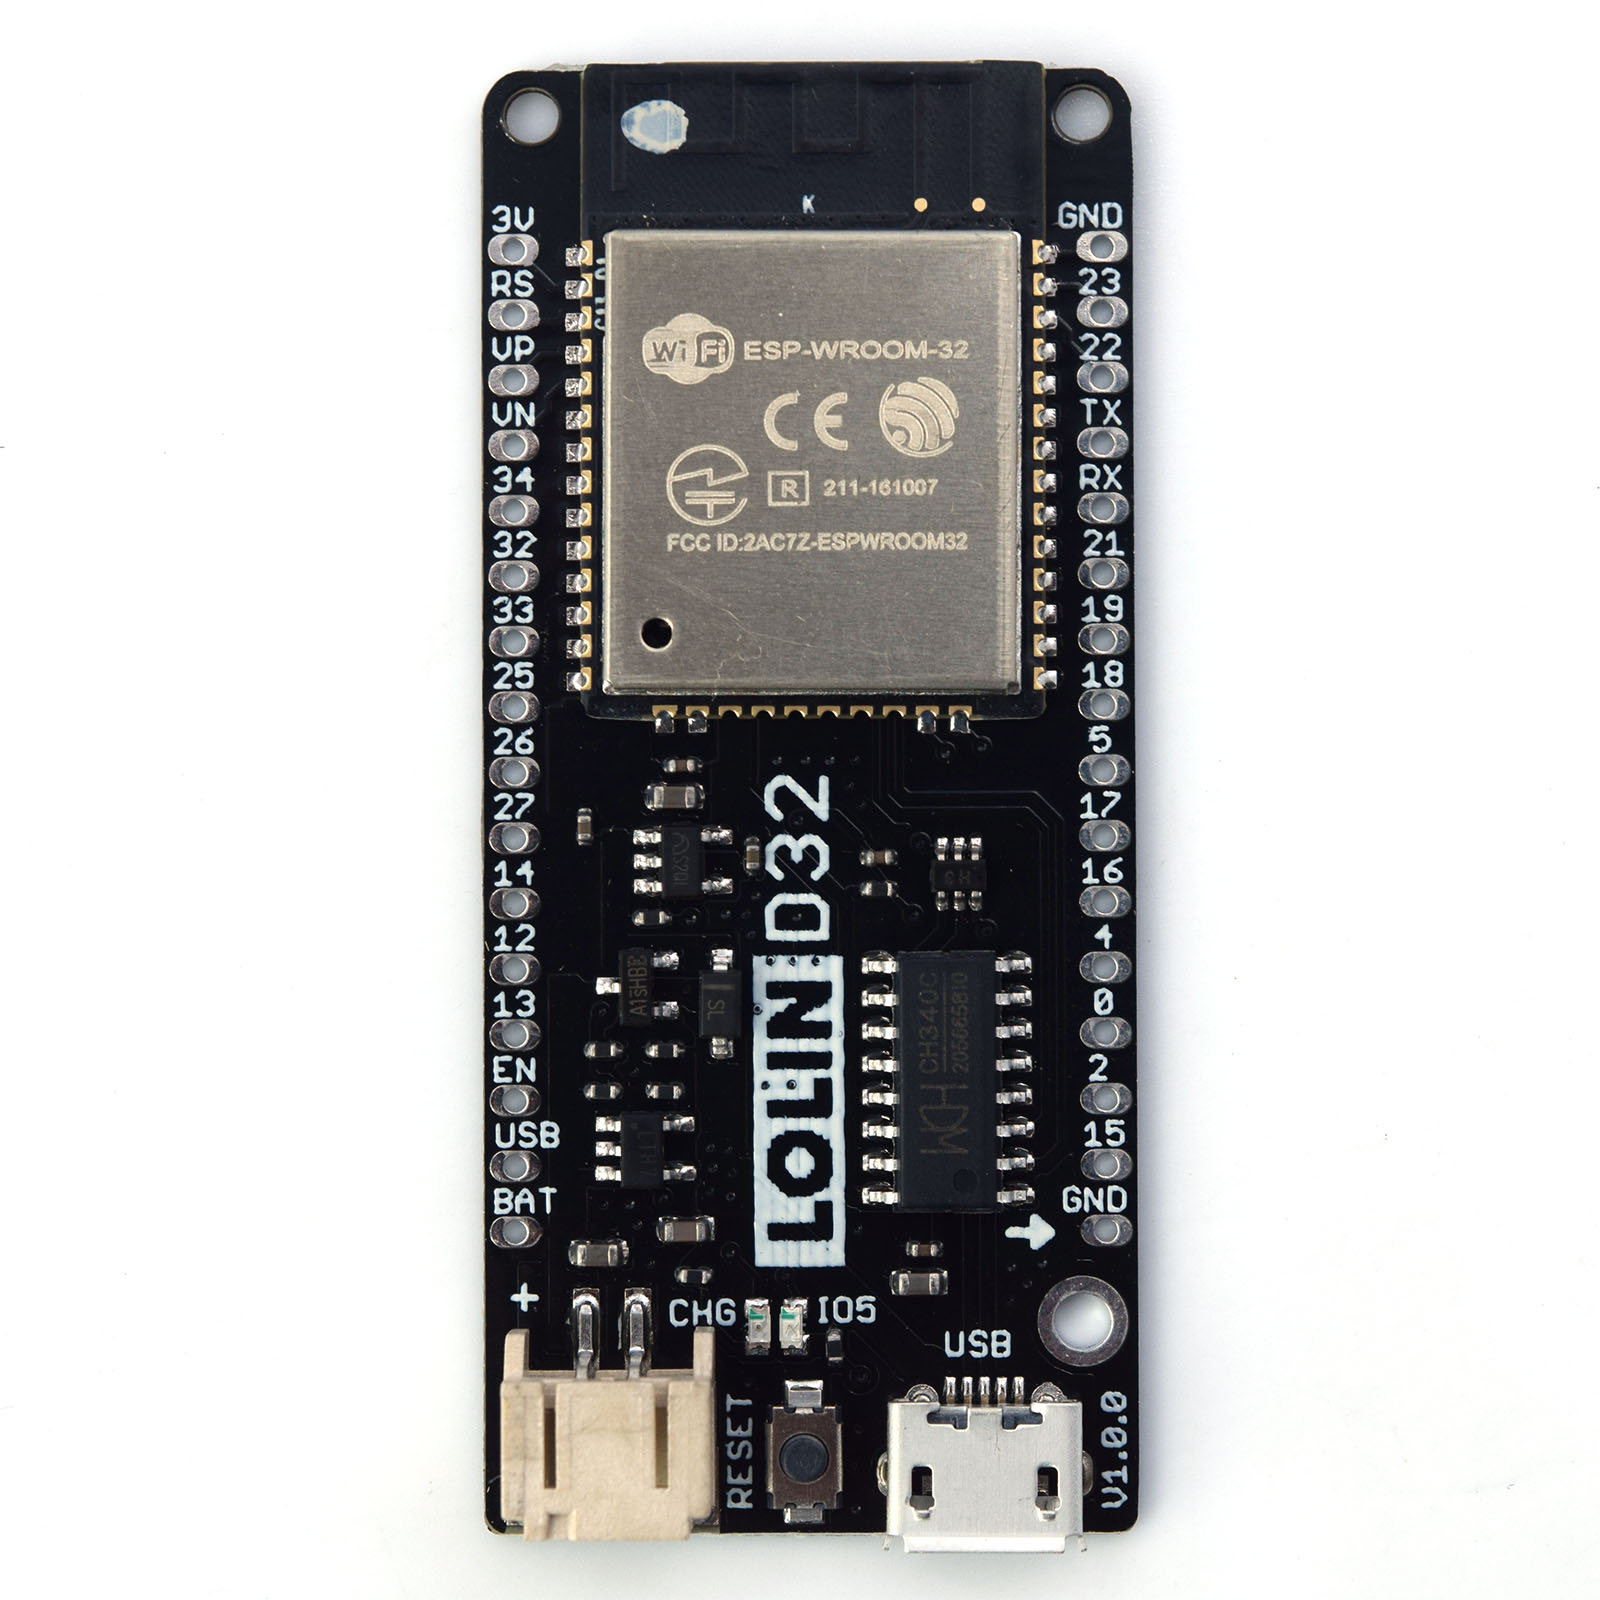
\includegraphics[scale=0.5]{images/d32_lolin}
    \caption{ESP32 pločica (Izvor:~\cite{wemos-docs})}
\end{figure}

Uz glavnu pločicu potreban je i takozvani \textit{power shield} koji omogućava napajanje od 12V\@.
Komponenta nije uključena u standardni paket WEMOS D32, a potrebna je zbog električne brave koja radi na 12V\@.

\pagebreak

\subsection{MFRC522}

Kreditne kartice sadrže RFID čip u kojem je pohranjen jedinstveni identifikator kartice (UID).
Za autorizaciju pristupa sefu potrebno je pročitati UID s čitačem RFID kartica.

\begin{figure}[h!]
    \centering
    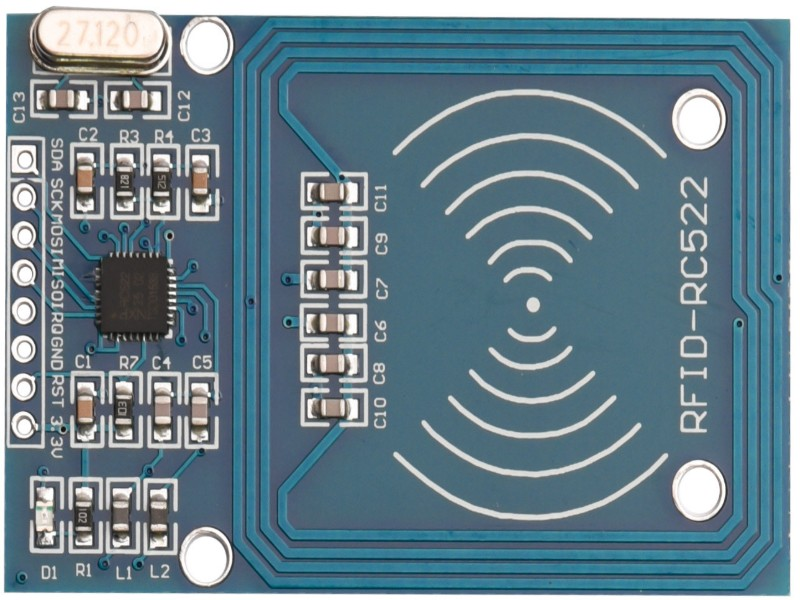
\includegraphics[scale=0.25]{images/mfrc522}
    \caption{MFRC522 čitač (Izvor:~\cite{mfrc522-eradionica})}
\end{figure}

\subsection{Mikroprekidač}

Magnetski mikroprekidač je dvodijelna komponenta koja zatvara strujni krug kad su obje komponente blizu jedna drugoj
(oko 20 milimetara).
Jednostavna komponenta koja služi pri određivanju stanja sefa (otvoren ili zatvoren).
Proizvođač je tvrtka \textit{SparkFun}.

\begin{figure}[h!]
    \centering
    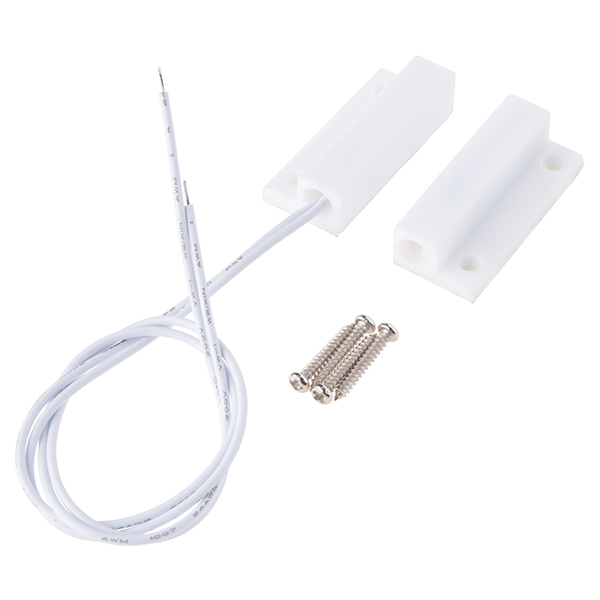
\includegraphics{images/magnetic-switch}
    \caption{Magnetski mikroprekidač (Izvor:~\cite{sparkfun-switch})}
\end{figure}

\pagebreak

\subsection{RGB LED}

LED dioda koja podržava RGB spektar boja.
Komponenta služi kao informacija korisniku o uspješnosti otvaranja sefa.

\begin{figure}[h!]
    \centering
    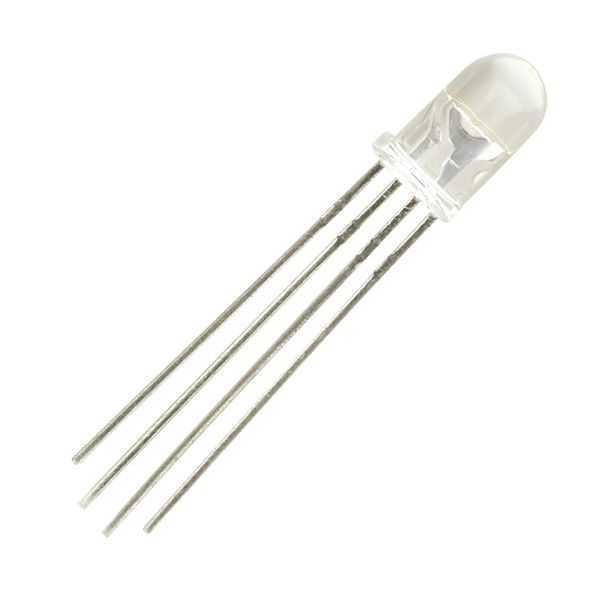
\includegraphics[scale=0.7]{images/rgb-led}
    \caption{RGB LED (Izvor:~\cite{robotistan-led})}
\end{figure}

\subsection{Brava i relej}

Električna brava koja radi na 12V i 500mA\@.
Kad relej zatvori strujni krug brava se otvara i omogućava korisniku pristup sefu.

\begin{figure}[h!]
    \centering
    \begin{subfigure}{.5\textwidth}
        \centering
        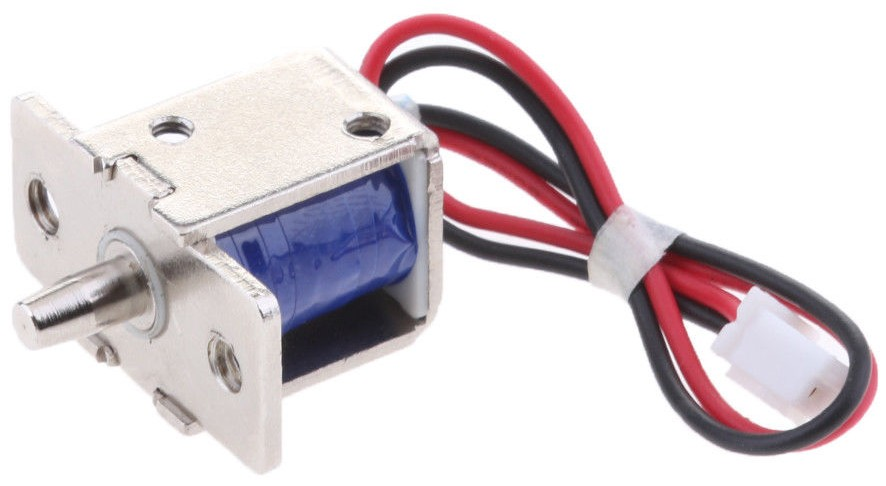
\includegraphics[width=.4\linewidth]{images/door-lock}
        \caption{Brava (Izvor:~\cite{ebay-doorlock})}
    \end{subfigure}%
    \begin{subfigure}{.5\textwidth}
        \centering
        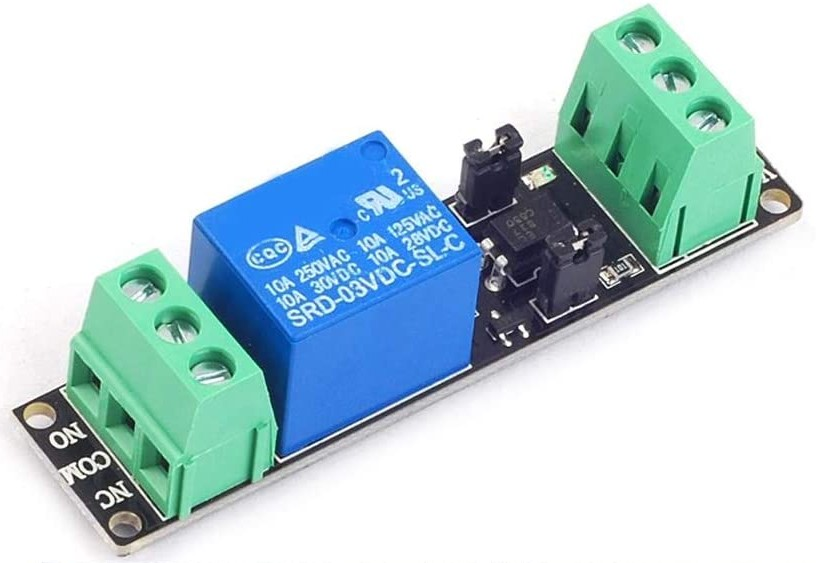
\includegraphics[width=.4\linewidth]{images/relay}
        \caption{Relej (Izvor:~\cite{amazon-relay})}
    \end{subfigure}
\end{figure}

\subsection{Napajanje}

\begin{wrapfigure}{r}{0.5\textwidth}
    \centering
    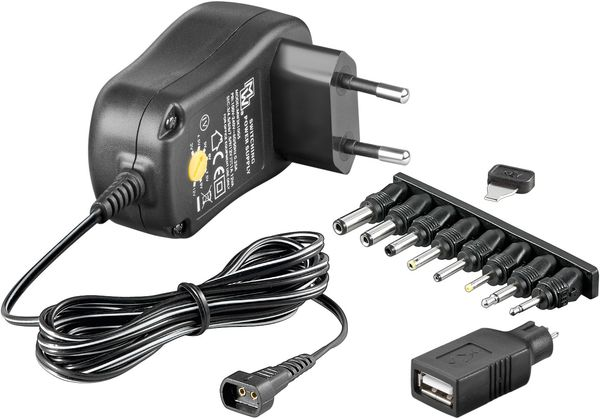
\includegraphics[scale=0.4]{images/power-supply}
    \caption{Napajanje (Izvor:~\cite{chipoteka-power-supply})}
\end{wrapfigure}

Većina komponenti zahtjeva 3.3V napajanje, no električna brava radi na 12V pa zahtjeva vanjsko napajanje.
Potrebno je vanjsko napajanje koje pretvara 220V u 12V\@.

\clearpage

\subsection{Schema komponenti}

\begin{figure}[h!]
    \centering
    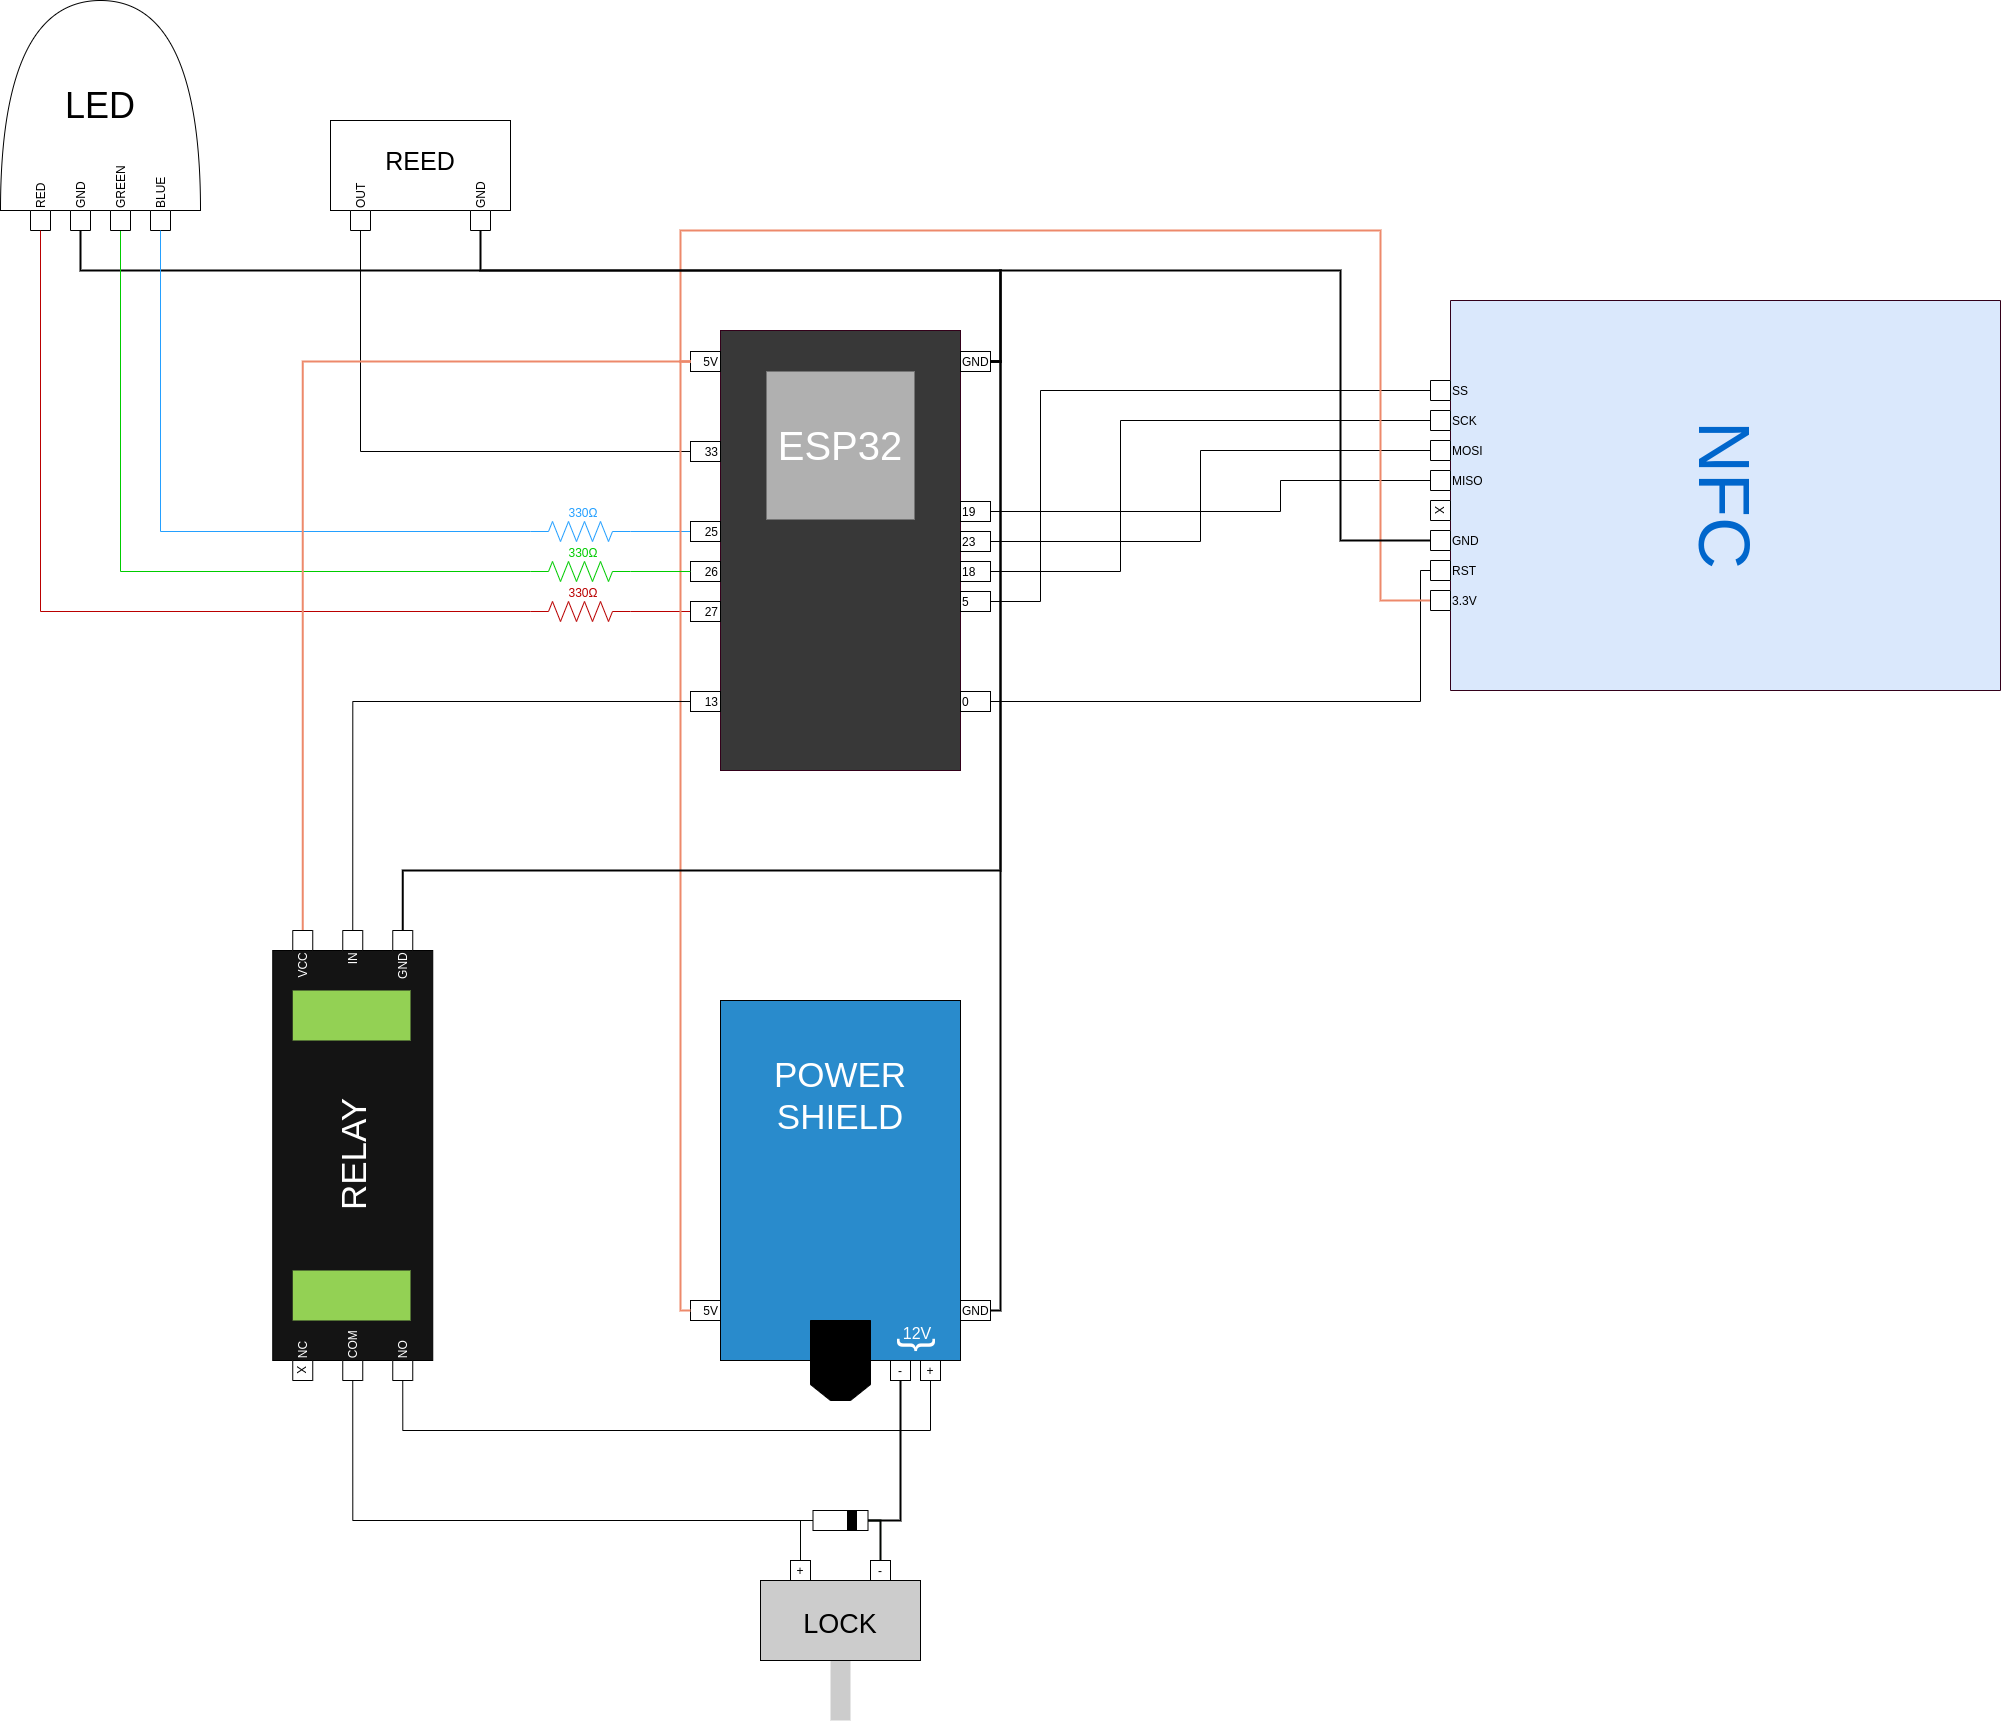
\includegraphics[width=\textwidth]{images/component-schema}
    \caption{Schema komponenti}
    \label{fig:component-schema}
\end{figure}

Na slici~\ref{fig:component-schema} u centru svega nalazi se ESP32 mikrokontroler.
Pinovi s desne strane mikrokontrolera (19, 23, 18, 5 i 0) potrebni su za komunikaciju s NFC čitačem.
Sve tri boje LED diode (crvena, zelena i plava) su u upotrebi, a između svake žice i mikrokontrolera nalazi se
otpornik od 300 oma.
Magnetski mikroprekidač najjednostavnija je komponenta, a informacije o stanju pruža mikrokontroleru na pinu broj 33.
Upravljanje bravom se ne izvodi direktno već pomoću releja na pinu broj 13.
Relej i brava zahtijevaju napajanje i uzemljenje od 12V s \textit{power shield-a}.
Dovodom struje na \textit{IN} ulaz releja zatvara se strujni krug i propušta se struja na \textit{COM} izlaz koji je
povezan s pozitivnim polom brave i otključava bravu.

Testiranjem sefa utvrđeno je neočekivano ponašanje.
Uzastopno otključavanje brave dovodi do nemogućnosti čitanja kartice i podataka s iste.
Ispitivanjem je utvrđeno da mikrokontroler radi pravilno, dok NFC čitač ne prepoznaje ranije prepoznatu karticu.
Nema uzorka u pojavljivanju ovakvog ponašanja (npr.\ nakon X uspješnih čitanja ili X minuta dolazi do nepravilnog rada)
već se događa nasumično.

Brava uvlači klin pomoću elektromagnetske induktivne zavojnice.
Dovodom struje na zavojnicu električna energija se pretvara u magnetsku i tvori magnetsko polje.
Odvodom struje s polova brave magnetsko polje se ruši i stvara naponski impuls obrnutog polariteta~\cite{flyback-diode}.
Elektroni promjene smjer kretanja i, na sreću, samo privremeno poremete rad NFC čitača.
Nemoguće je spriječiti promjenu smjera kretanja, no moguće je ograničiti kretanje.
Za to je potrebna takozvana \textit{flyback} dioda koja propušta jedan smjer, a blokira obrnuti smjer kretanja
~\cite{flyback-diode}.
Na slici~\ref{fig:component-schema} kod kontakata brave nalazi se \textit{flyback} dioda.
Na taj način elektroni s obratnim smjerom kretanja ne dolaze do ostalih komponenti sefa i NFC čitač radi pravilno.

\subsection{Integracija komponenti u sef}

Mikrokontroler, \textit{power shield}, relej, \textit{flyback} dioda i ožičenje zalemljeni su na plastičnu pločicu,
a pločica je pričvršćena za kutiju.
NFC čitač, brava i utor za bravu, mikroprekidač i RGB LED dioda direktno su pričvršćeni za kutiju.

\begin{figure}[h!]
    \centering
    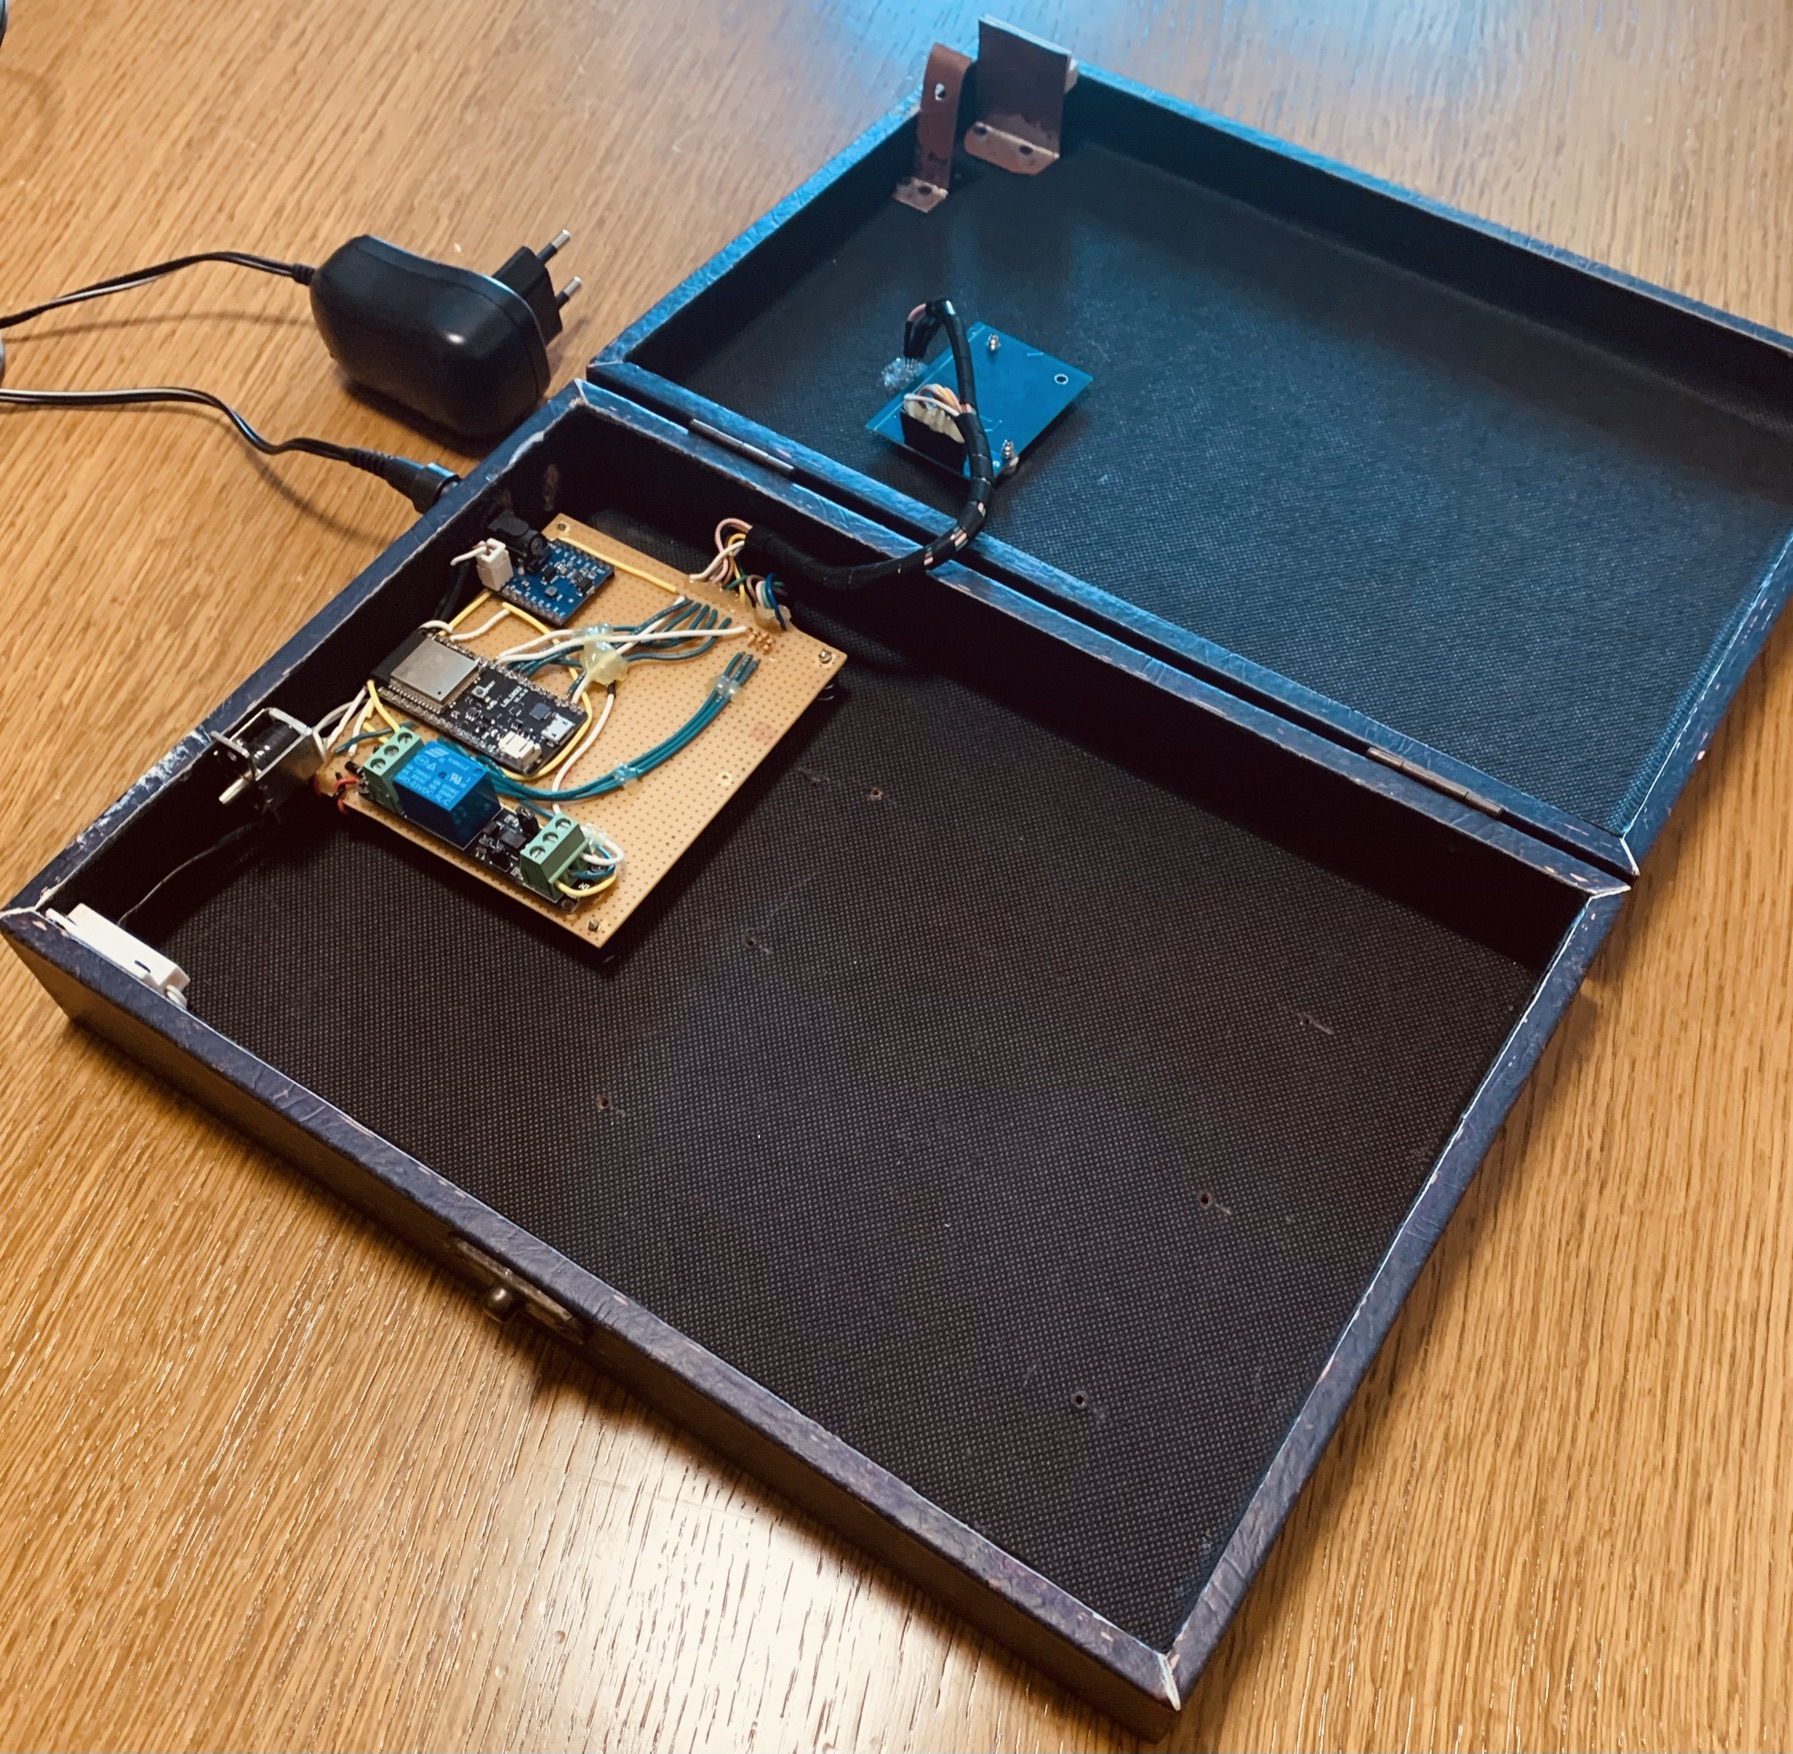
\includegraphics[width=\textwidth]{images/integrated-components}
    \caption{Komponente integrirane u kutiju}
\end{figure}



\chapter{Zaključak}

\ldots


\printbibliography[title=Popis literature]
\addcontentsline{toc}{chapter}{Popis literature}

\listoffigures
\addcontentsline{toc}{chapter}{Popis slika}
 
\listoftables
\addcontentsline{toc}{chapter}{Popis popis tablica}

\appendix
\renewcommand{\thechapter}{\arabic{chapter}}

\end{document}
